\chapter{Introduction}

Recently, mobile devices become more and more important in people's life. At the same time, some location/context based tools and apps are developed, which are very useful. For example, a mobile phone can automatically turn itself into silent mode while in a meeting. A portable audio player can play appropriate musics in different scenes. Thus, scene recognition attracts more and more attention.

The audio effects, such as {\em phone-ringing}, {\em car-horn}, etc., play a important role in our daily life. Comparing with other data, such as image data and video data, audio data is much more easier to get. For example, mobile phone can capture audio information from all around, all directions. Besides, audio data can record a lot of information related to scene/activity/context.

Therefore, audio data can be used to infer/recognize/classify current scene/activity/context. Although this work is similar to speech recognition, there are lots of differences. For example, speech has the limited size of phonemes as natural basic units, while environmental sound does not have them. Thus, understanding environmental sound and infer the scene is still an open problem.

In early listening test conducted in \cite{peltonen2001recognition}, human beings are able to recognize daily scenes in $70\%$ accuracy on average, and confusions come among those contexts that shares some same prominent audio events. Therefore, we can conclude that for human beings, the audio events are the most important part to recognize audio context.

Some previous work \cite{1621215, heittola2010audio} used the audio events to do scene recognition. All of their work obtained a good accuracy. However, they chose the audio events and labeled them manually, and might not have good expansion.

In this thesis, we propose an event-based audio scenes recognition system using knowledge bases. Our approach assumes that different audio scenes can be distinguished by some audio events. The main contributions of our work are:
\begin{itemize}
\item We use knowledge base and text data to build the probabilistic model of audio events and scenes rather than using audio data directly. Thus our model can be more precise, since it is much easier to find a huge number of text data than audio data. Also, text processing is much faster than audio processing.
\item Our system can download and label training data automatically, instead of doing manual work. All of our training data are download directly from Internet without manual pre-precessing. Therefore, our system is more scalable than previous work.
\item We propose a method to cluster audio training data. After clustering, we use different model to describe different cluster, which can reduce the impact of low quality data.
\end{itemize}

Our system is designed as figure \ref{fig:sys}. We will introduce each part in next chapters.
\begin{figure}[!htb]
\centering
\includegraphics[width=0.8\textwidth]{figures/all.eps}
\caption{Design of our scene recognition system}
\label{fig:sys}
\end{figure}


